\section{Frontend}

L'application en l'état est disponible et jouable par toutes et tous à l'adresse suivante \href{https://place.beescreens.ch}{place.beescreens.ch}. Il s'agit de la version en production déployée sur la machine virtuelle \gls{beescreens}.

\subsection{Présentation de l'interface}

Voici tout d'abord quelques figures présentant l'interface sur ordinateur ainsi que sur mobile. La différence principale entre les deux versions est le menu permettant à l'utilisateur de choisir la couleur de son pixel.


\begin{figure}[H]
  \centering
  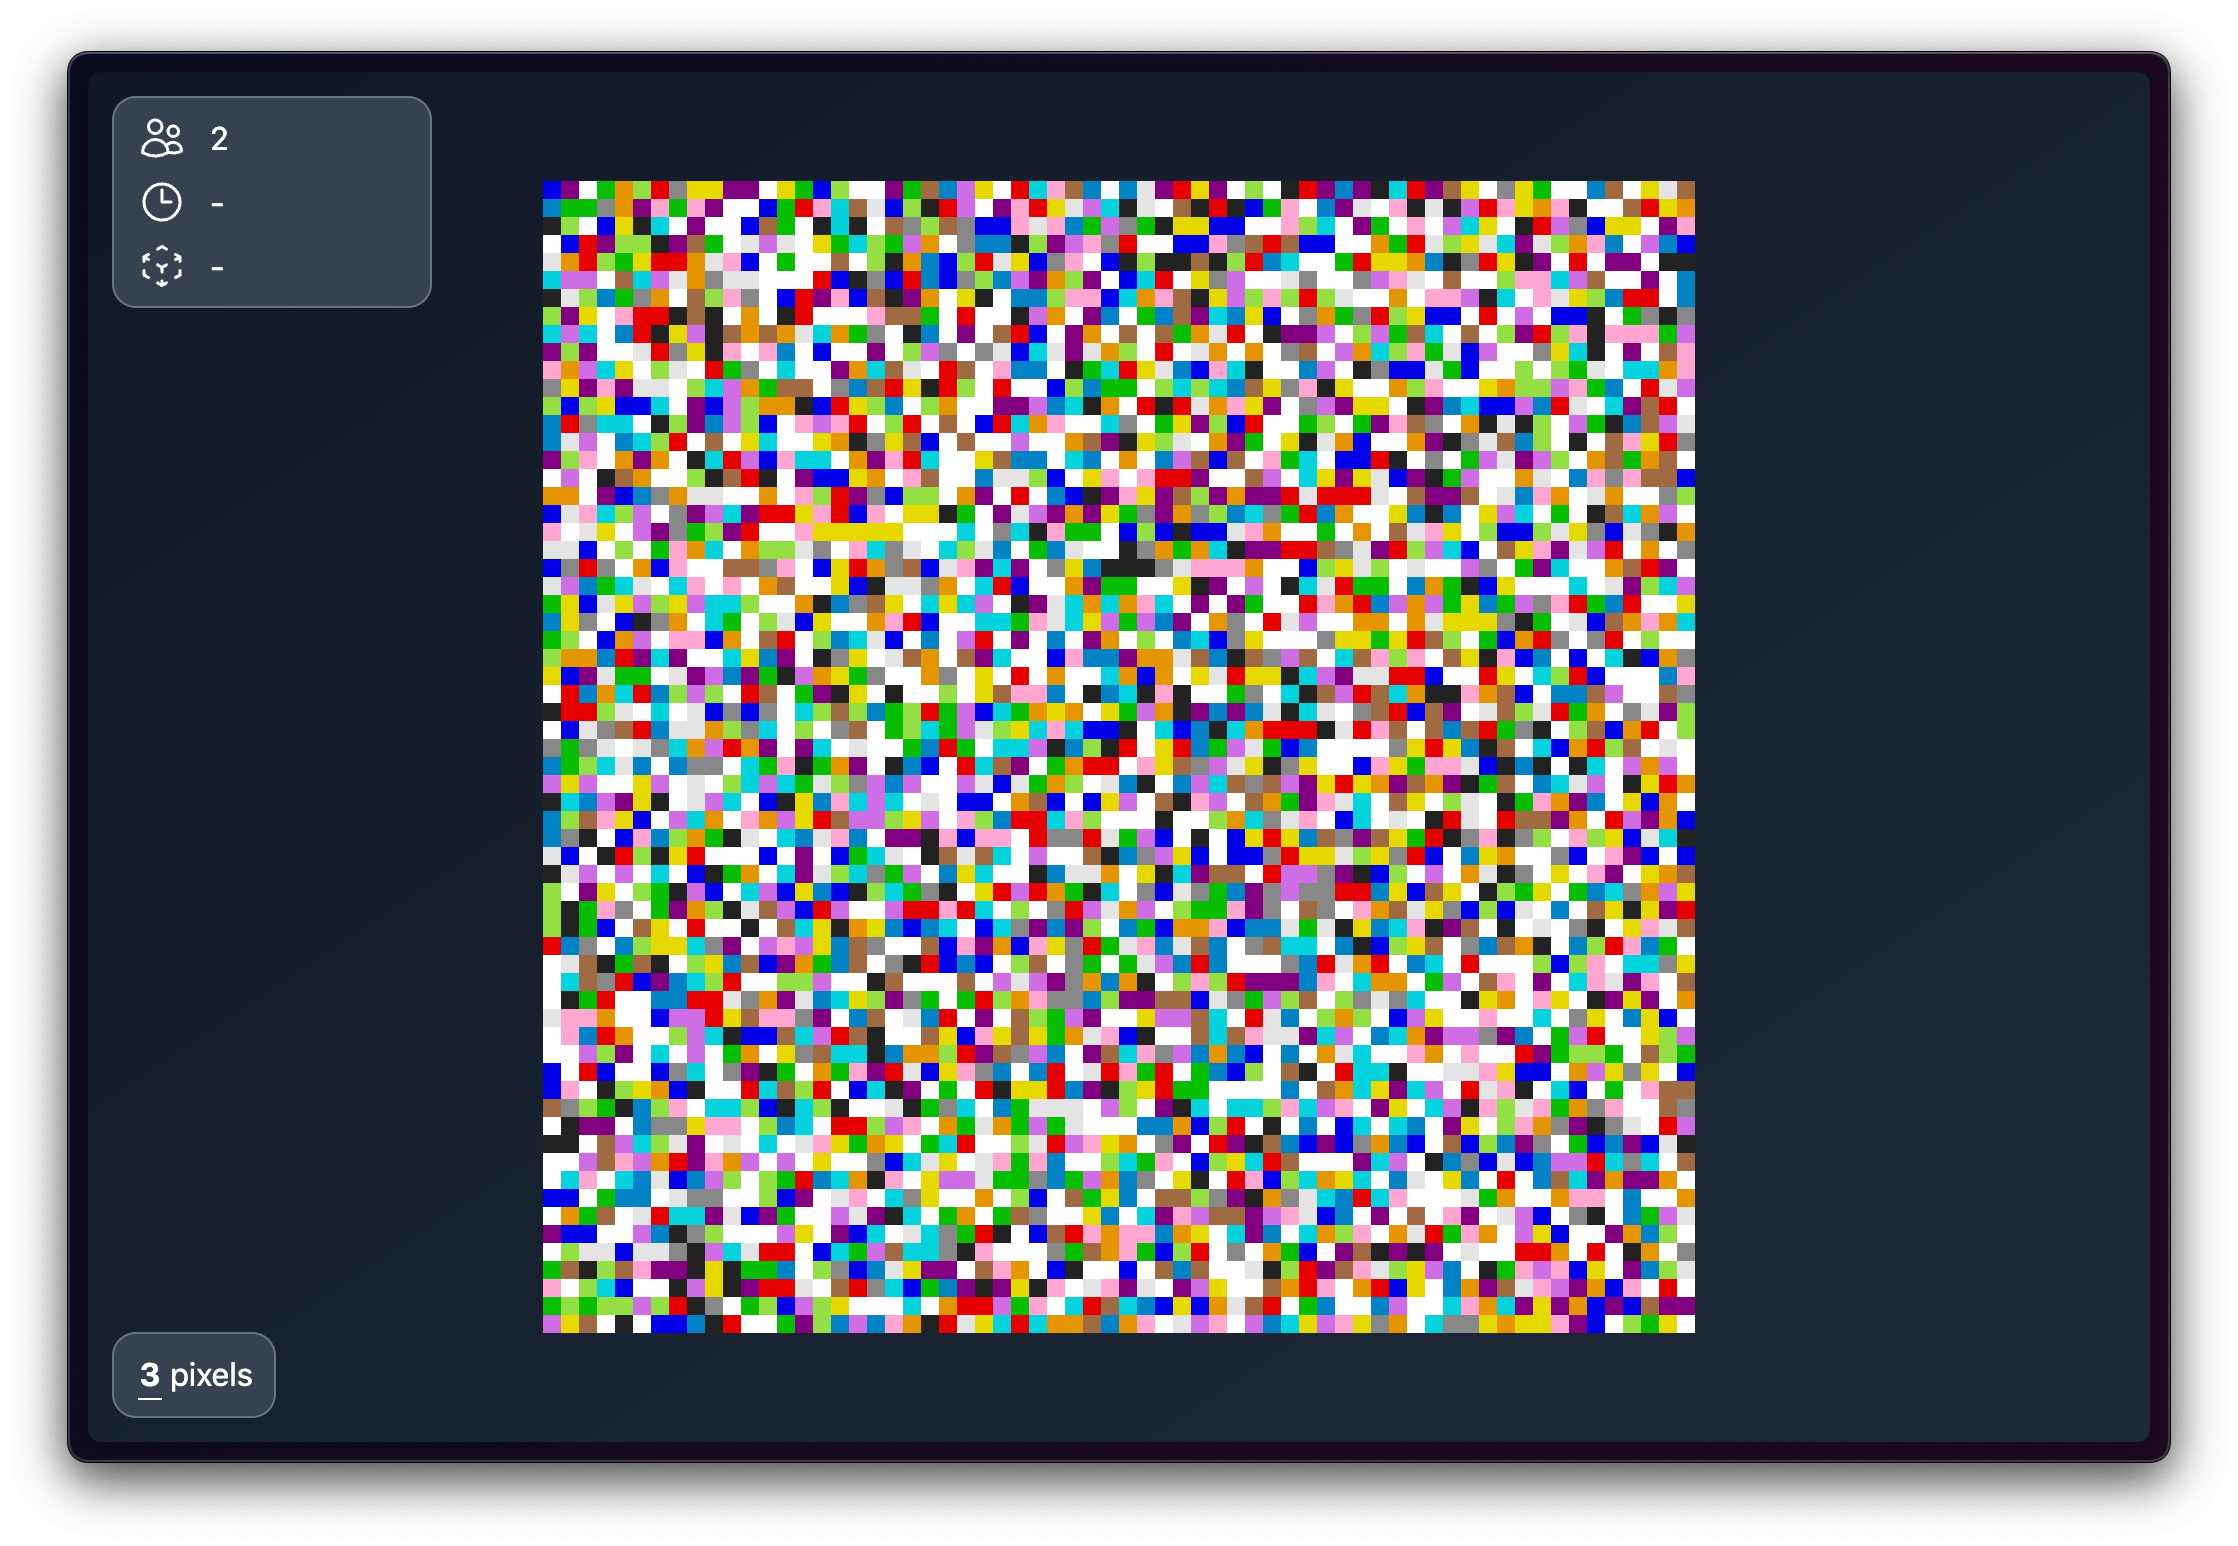
\includegraphics[width=1\textwidth]{./assets/figures/screenshot-app-v2-1.png}
  \caption{Interface de BeePlace sur ordinateur à l'arrivée sur la page}
  \label{fig:screenshot-app-1}
\end{figure}

\begin{figure}[H]
  \centering
  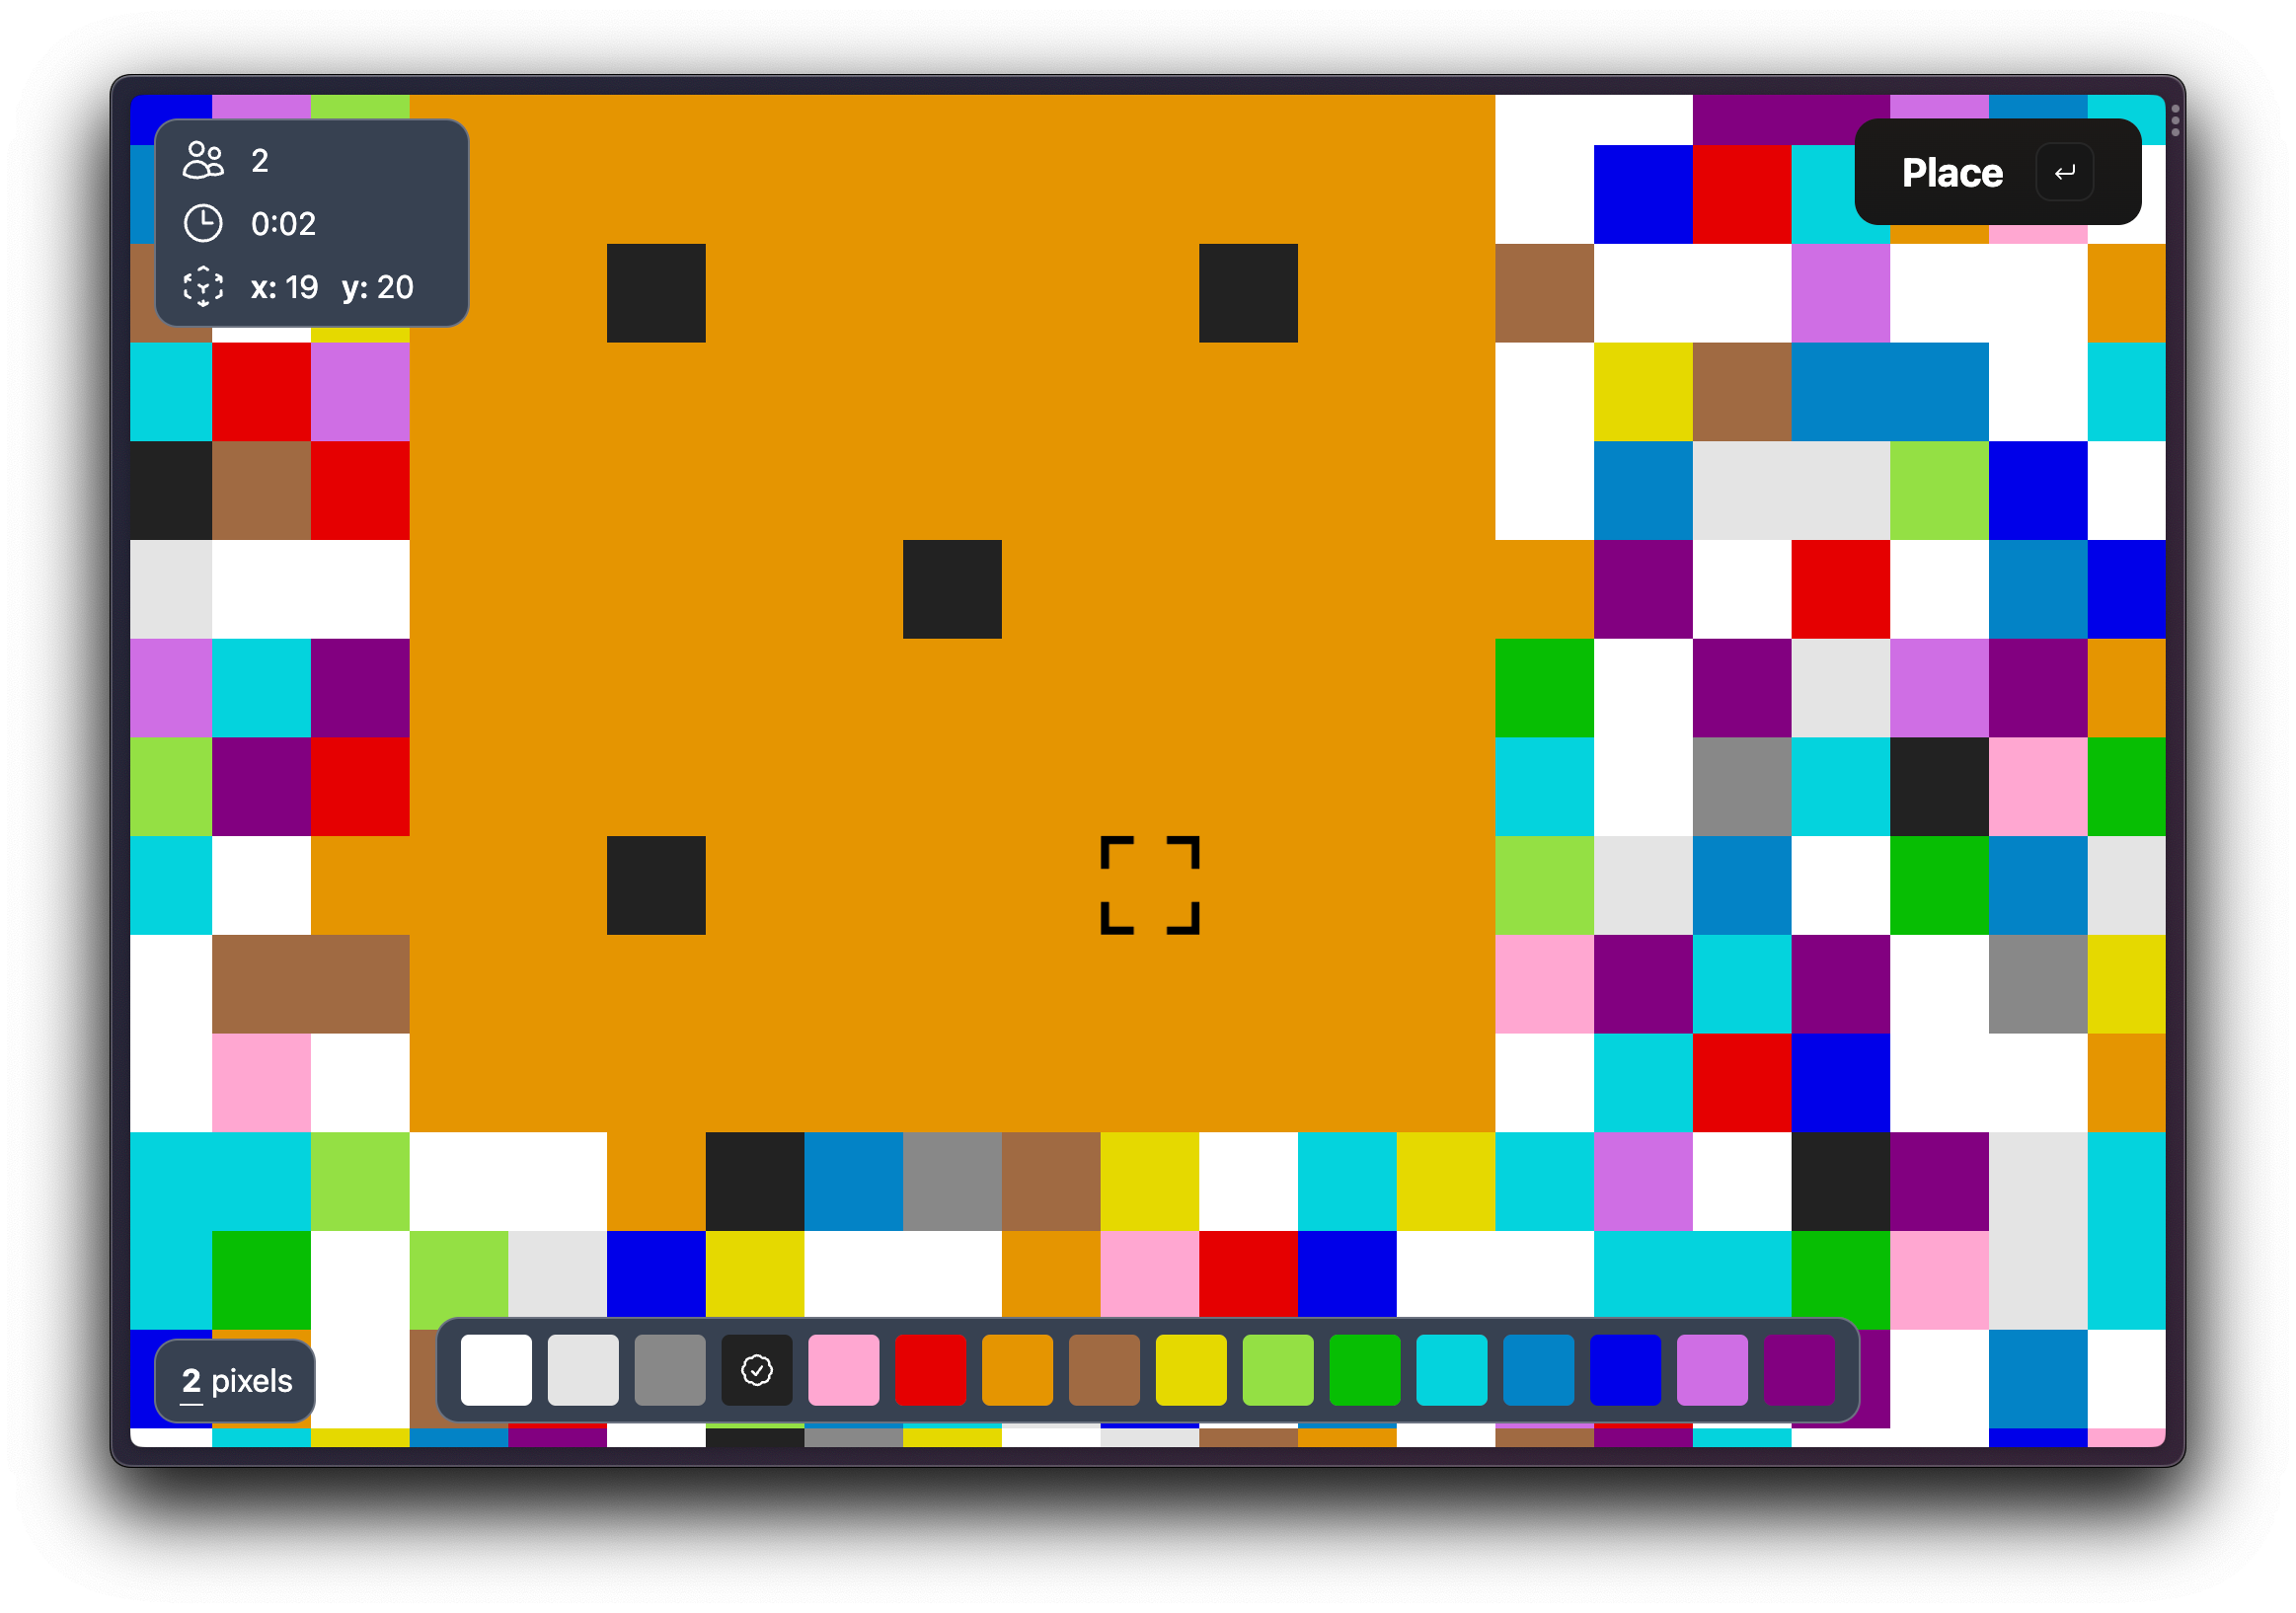
\includegraphics[width=1\textwidth]{./assets/figures/screenshot-app-v2-2.png}
  \caption{Interface de BeePlace sur ordinateur lorsque l'utilisateur clique sur un pixel}
  \label{fig:screenshot-app-2}
\end{figure}

\begin{figure}[H]
  \centering
  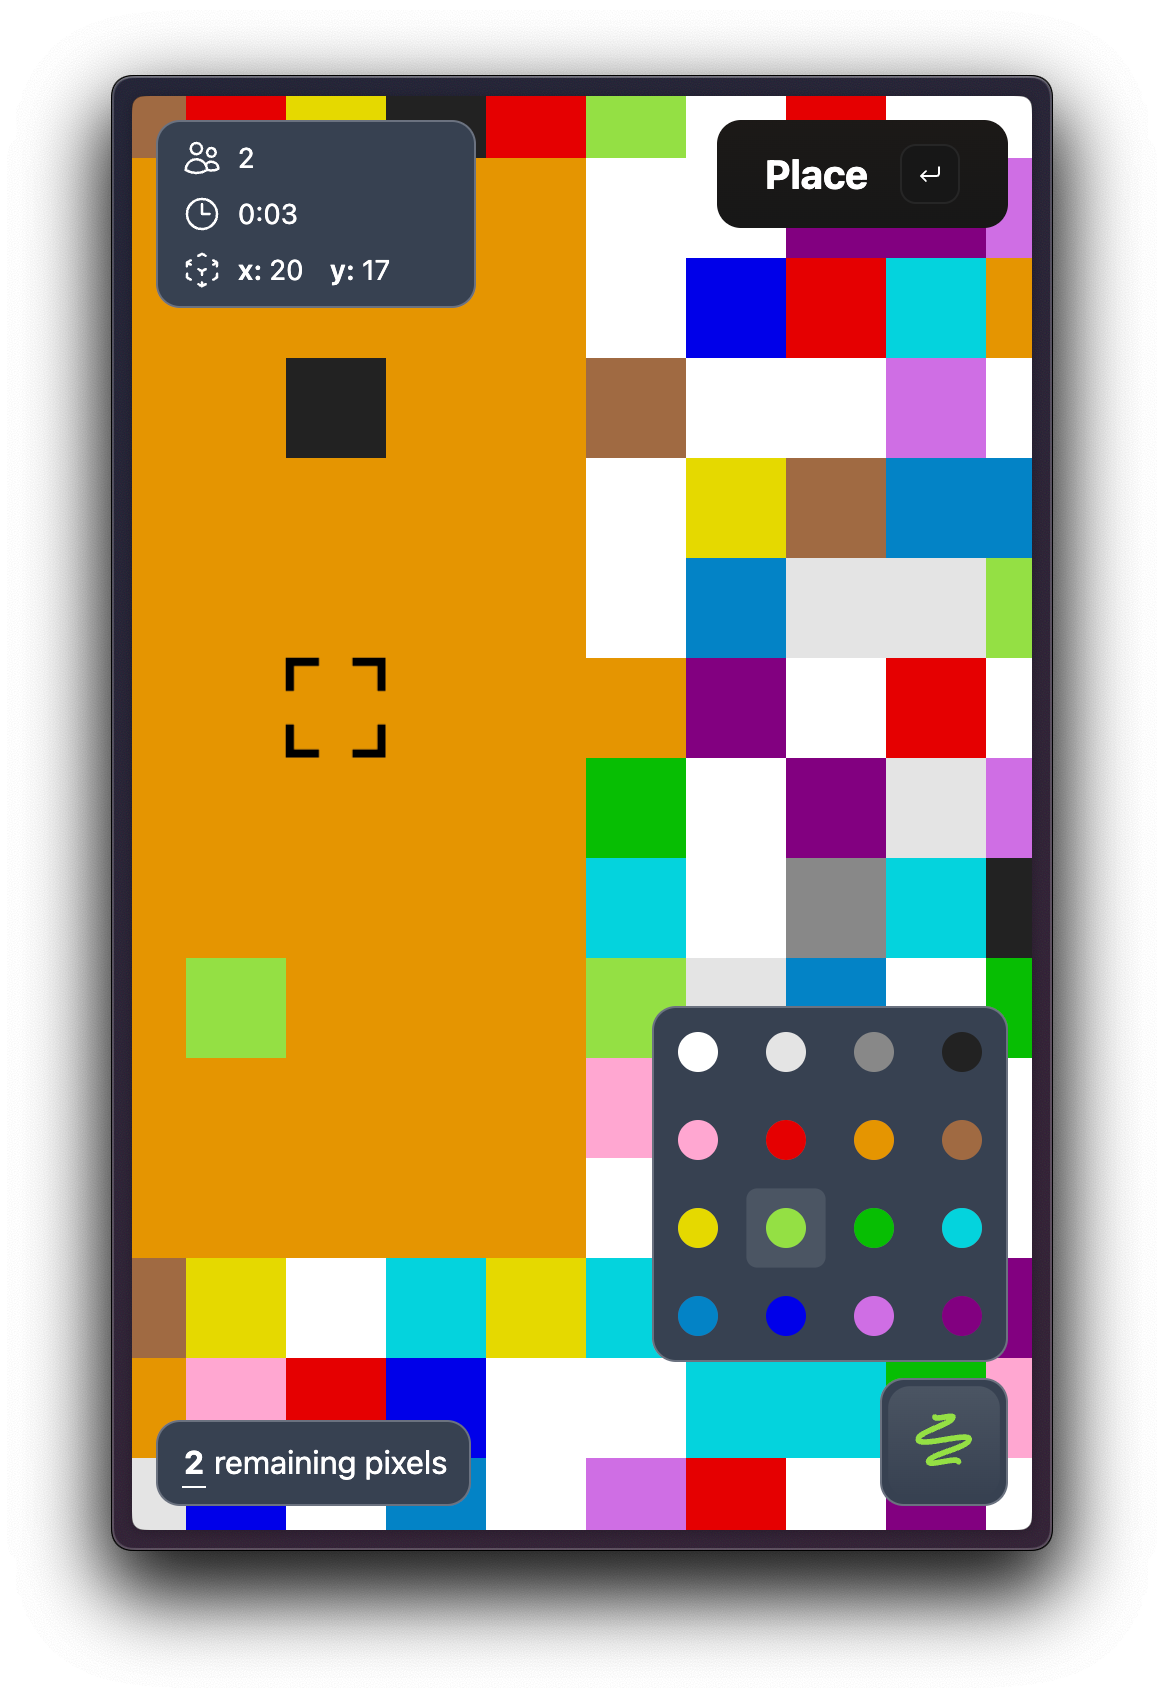
\includegraphics[width=0.5\textwidth]{./assets/figures/screenshot-app-v2-3.png}
  \caption{Interface de BeePlace sur mobile}
  \label{fig:screenshot-app-3}
\end{figure}

\subsection{Canvas}

La toile est le point central de l'application, celle-ci est modélisée grâce à l'élément HTML5 \mintinline[breaklines]{bash}{<canvas>}~\cite{canvas}. Cet élément permet de dessiner des formes, des images et du texte. Il est possible de dessiner directement sur le canvas en utilisant le contexte 2D ou 3D. Les formes à dessiner sont très simples dans le cas de \gls{beeplace} car il s'agit de pixels représentés par des carrés de couleurs unies.

\subsubsection{Dessin des pixels}

Deux choix sont possibles pour dessiner les pixels sur le canvas:

\begin{enumerate}
  \item Représenter un pixel comme un pixel du canvas;
  \item Représenter un pixel comme un carré de plusieurs pixels du canvas.
\end{enumerate}

La deuxième variante permet d'avoir directement une représentation de meilleure résolution de la toile. En effet, si la toile a par exemple des dimensions de 64 pixels de largeur, l'utilisateur ne doit pas avoir un canvas de 64 pixels affiché à l'écran, ce qui serait trop petit et illisible. Cependant, représenter un pixel par plusieurs pixels sur le canvas pose problème lorsque l'utilisateur clique sur le canvas pour placer un pixel. En effet, cela demanderait plus de calculs pour connaître les coordonnées réelles du clique de l'utilisateur. La première variante a donc été choisie. Afin de ne pas avoir un canvas trop petit, il est possible de zoomer sur l'élément via la propriété transform en CSS~\cite{transformcss}. De base, cela rendrait l'image floue mais il est possible de changer ce comportement en utilisant l'attribut image-rendering~\cite{image-renderingcss} avec comme valeur \mintinline[breaklines]{bash}{pixelated}. Comme notre toile est remplie de pixels, cela permet d'avoir un rendu parfaitement net.

\subsection{PinchZoom}

Écouter les événements utilisateurs pour réaliser des transformations sur un élément (le déplacer, zoomer à un point précis) revient à réaliser ce qu'on appelle un "Pinch-to-Zoom" ou plus simplement "PinchZoom". Ce terme signifie littéralement "pincer pour zoomer". Il s'agit d'un geste utilisé sur les appareils tactiles pour zoomer sur une image ou une page web ainsi que se déplacer. Réaliser une implémentation de ce geste devient vite une tâche fastidieuse. En effet, il est nécessaire d'écouter divers événements différents pour que l'utilisation soit agréable sur tout type d'appareils:

\begin{itemize}
  \item Les événements de la souris;
  \item Les événements tactiles;
  \item Les événements du pavé tactile qui sont un mélange des deux précédents.
\end{itemize}

Adapter le code en fonction de la nature de l'événement devient vite compliqué et source de bug. Heureusement, plusieurs librairies existent afin de faciliter l'implémentation, surtout dans l'écosystème React très riche. La liste qui suit contient les options testées et les raisons pour lesquelles elles ont ou non été retenues.

\subsubsection{React-zoom-pan-pinch}

Le librairie la plus connue se nomme React-zoom-pan-pinch~\cite{react-zoom-pan-pinch}. Celle-ci propose un code assez léger, entièrement en \gls{typescript} et sans dépendance externe. Le problème survient lorsque l'utilisateur doit interagir avec l'élément à l'intérieur du PinchZoom, dans ce cas-ci le canvas. En effet, en plus de pouvoir déplacer et zoomer sur le canvas, l'utilisateur doit pouvoir cliquer sur celui-ci pour placer un pixel. Cependant, la librairie ne permet pas de le faire nativement et un comportement très étrange de translation en dehors de l'écran se produit lors d'un clique. C'est pourquoi cette librairie n'a pas été retenue.

\subsubsection{React-quick-pinch-zoom}

Cette seconde librairie, react-quick-pinch-zoom~\cite{react-quick-pinch-zoom} est une adaptation pour React d'une librairie \gls{javascript} plus connue nommée simplement PinchZoom.js~\cite{pinchzoomjs}. Le soucis de cette libraire survient lorsque l'élément à l'intérieur du PinchZoom doit prendre toute la taille de la fenêtre, ce qui est le cas pour \gls{beeplace}: le canvas est l'élément unique de l'application et prend donc l'intégralité de la page. Lorsque c'est le cas, le comportement de la librairie est étrange et très aléatoire en fonction des événements utilisateurs. Cette seconde librairie n'a donc également pas été retenue.

\subsubsection{React-fast-pinch-zoom}

Heureusement, le même auteur que la seconde librairie a développé une autre version appelée react-fast-pinch-zoom~\cite{react-fast-pinch-zoom}. Celle-ci se base cette fois-ci sur une librairie de PinchZoom réalisée par l'équipe de Google Chrome~\cite{pinch-zoom-googlechromelabs}. Celle librairie repose elle-même sur une autre libraire de la même équipe Google Chrome, PointerTracker~\cite{pointer-tracker}. L'avantage de cette librairie est qu'elle utilise la notion de Pointer events~\cite{pointer-events} qui, contrairement aux anciens événements d'interaction, ne partent pas du principe que l'utilisateur utilise une souris. En effet, ces Pointer events sont utilisés pour tous les appareils, que ce soit une souris, un écran tactile ou un pavé tactile.

Malheureusement la librairie, react-fast-pinch-zoom~\cite{react-fast-pinch-zoom}, est écrite dans une ancienne manière de faire du React nommée Class component. L'équipe React elle-même recommande d'utiliser des composants en fonction plutôt que des classes "We recommend defining components as functions instead of classes."~\cite{react-class-component}. C'est pour cette raison que le code de la librairie a été copié dans le projet et adapté pour être utilisé avec des composants en fonction.

\subsection{Gestion du state}

L'application React doit garder en tout temps un état à jour. Cet état comporte plusieurs éléments:

\begin{itemize}
  \item Les réglages initiaux de la toile comme sa taille, les couleurs disponibles, le temps d'attente entre chaque pixel, etc;
  \item Le nombre de pixels posés par l'utilisateur dans l'intervalle de temps;
  \item Le moment où l'utilisateur pourra à nouveau placer un pixel.
\end{itemize}

Toutes ces variables sont utilisées dans de nombreux composants React. Il est donc nécessaire de les stocker dans un endroit centralisé afin de pouvoir les utiliser facilement sans devoir les faire passer sur plusieurs niveaux d'imbrication. Pour cela, il existe principalement deux solutions:

\begin{enumerate}
  \item Utiliser une librairie externe de stockage de state.
  \item Utiliser le state fourni par React dans un Contexte~\cite{react-context} afin de le rendre accessible à tous les composants enfants.
\end{enumerate}

\subsubsection{Librairie externes}

De nombreuses librairies existent pour gérer le state d'une application React. La plus connue est Redux~\cite{react-redux}. Cependant, Redux est une librairie assez lourde et complexe à mettre en place. Elle est également très verbeuse. Il existe des alternatives plus légères et simples comme Zustand~\cite{zustand}.

Les avantages de Zustand sur Redux sont les suivants:
\begin{itemize}
  \item Plus simple et sans opinion donc plus facile à prendre en main.
  \item Zustand utilise les hooks de React comme moyen principal de consommer le state, sa syntaxe est donc plus proche de React.
  \item Zustand peut modifier le state sans forcer le composant à se re-rendre, ce qui peut être utile au niveau des performances.
\end{itemize}

\subsubsection{Contexte React}

Au lieu d'installer une libraire externe, il est possible d'utiliser le Contexte React~\cite{react-context}. Celui-ci permet de stocker des données ainsi que des fonctions utilitaires dans un endroit centralisé et de les rendre accessibles à tous les composants enfants. Cependant, les contextes amènent plusieurs problèmes:

\begin{itemize}
  \item Un contexte React n'est pas fait pour stocker des données qui changent souvent. En effet, à chaque changement de state, tous les composants enfants sont re-rendus, ce qui peut être problématique au niveau des performances.
  \item Créer un contexte est assez verbeux et nécessite beaucoup de code pour un résultat assez simple.
  \item Le state dans un contexte n'est pas toujours accessible et à jour. Dans des fonctions de callback d'événements par exemple ou d'événements WebSockets, il faut utiliser des astuces afin de pouvoir accéder au state.
\end{itemize}

C'est pourquoi il est préférable d'utiliser une librairie externe comme Zustand.

\subsection{Mode affichage}
\label{display-mode}

Comme discuté rapidement dans le chapitre \ref{poc}, Proof of concept, il est nécessaire de pouvoir diviser l'affichage de l'application sur plusieurs écrans afin de pouvoir être projetée sur les tours de l'école. Ce mode est implémenté en deux parties:

\begin{itemize}
  \item Une page permettant de configurer les détails du mode affichage;
  \item Une page permettant d'afficher une partie de l'application.
\end{itemize}

\subsubsection{Configuration de l'affichage}

La configuration est disponible à l'adresse \texttt{/displays} comme la figure \ref{fig:display-mode-config} le montre. Il est possible de définir les paramètres suivants:

\begin{itemize}
  \item La largeur d'un écran en pixels;
  \item La hauteur d'un écran en pixels;
  \item Le nombre d'écrans en largeur;
  \item Le nombre d'écrans en hauteur.
\end{itemize}

Tous ces paramètres ont des valeurs par défaut configurée dans des variables d'environnement. Lorsque l'utilisateur en modifie un, la valeur est stockée dans le local storage du navigateur. Ainsi, la prochaine fois que l'utilisateur accède à la page de configuration, les valeurs sont déjà pré-remplies. L'interface de droite est mise à jour en temps réel afin de montrer à l'utilisateur à quoi ressemblera l'affichage.

L'utilisateur peut ensuite cliquer sur l'écran qu'il souhaite afficher et il sera redirigé vers la bonne page d'affichage.

\begin{figure}[H]
  \centering
  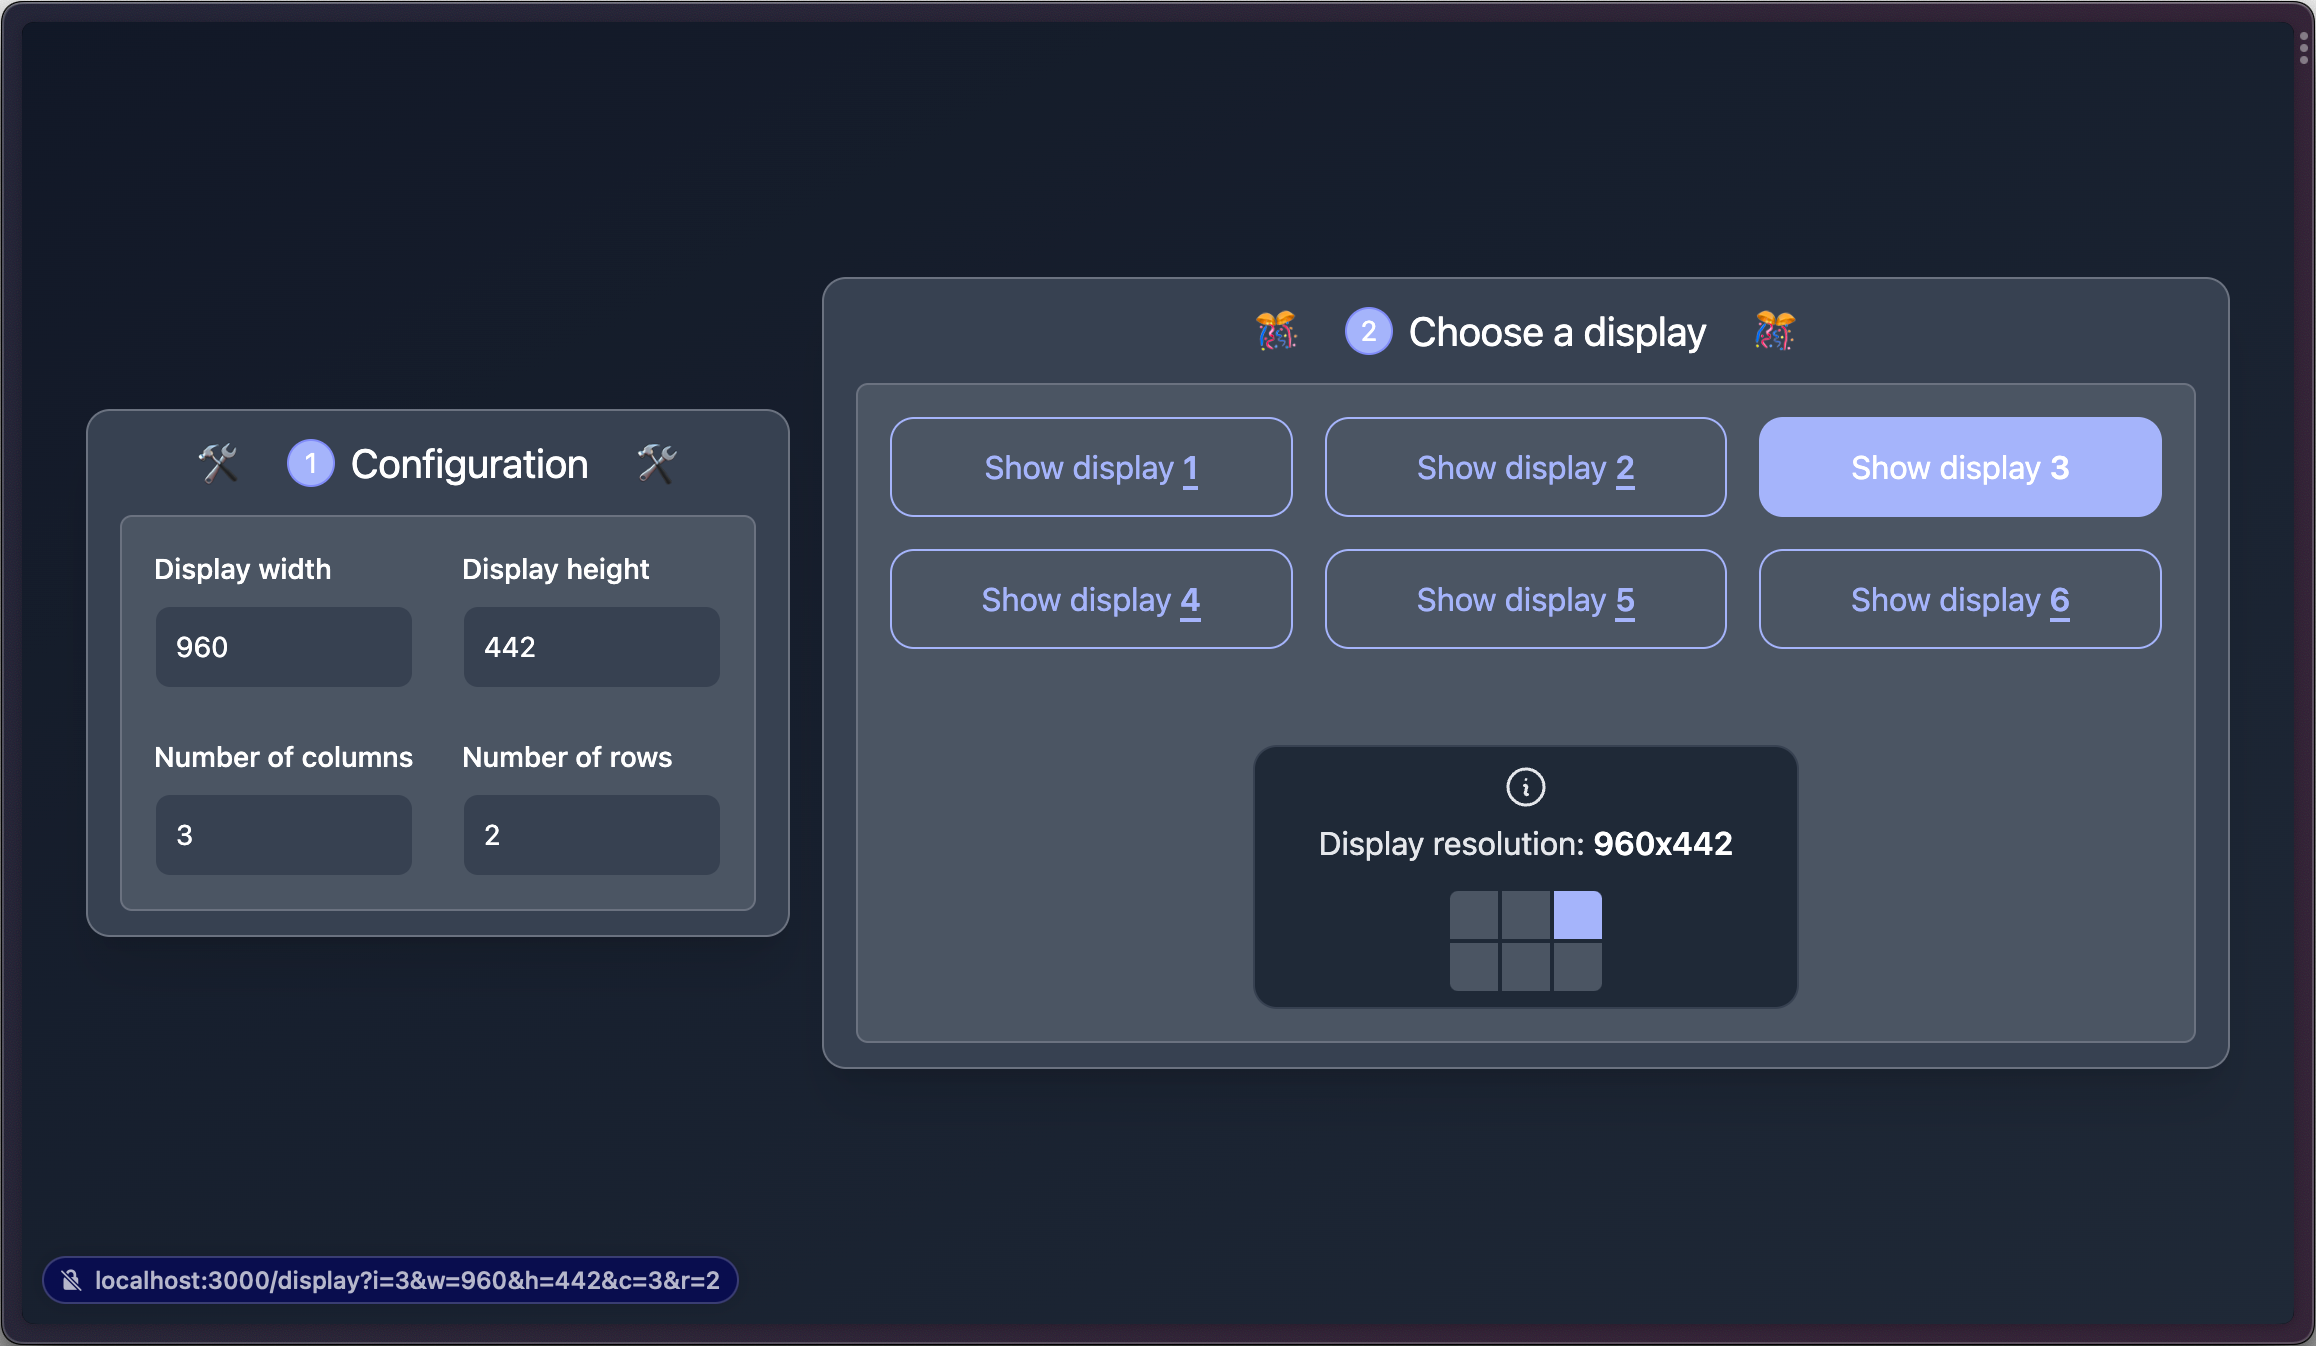
\includegraphics[width=1\textwidth]{./assets/figures/display-mode-config.png}
  \caption{Interface de configuration du mode affichage}
  \label{fig:display-mode-config}
\end{figure}

\subsubsection{Affichage d'une partie de la toile}

Une fois le lien cliqué, l'utilisateur est redirigé vers une page d'affichage contenant les bons paramètres dans l'URL, par exemple \texttt{/display?i=1\&w=504\&h=380\&c=3\&r=2}. La signification de ces paramètres est la suivante:

\begin{itemize}
  \item \texttt{i}: L'index de l'écran à afficher;
  \item \texttt{w}: La largeur d'un écran en pixels;
  \item \texttt{h}: La hauteur d'un écran en pixels;
  \item \texttt{c}: Le nombre d'écrans en largeur (nombre de colonnes);
  \item \texttt{r}: Le nombre d'écrans en hauteur (nombre de lignes).
\end{itemize}

La page s'occupe d'ensuite calculer la position et la dimensions de la toile afin de maximiser la taille de celle-ci. En effet, comme la toile est forcément carrée mais que les écrans sont souvent rectangulaires, il est nécessaire de calculer la plus grande taille possible pour la toile. La toile est donc centrée sur les écrans comme la figure \ref{fig:display-mode-example} le montre avec un exemple contenant six écrans.

Si l'utilisateur accède à la page \texttt{/display} sans paramètre, l'application se contente d'afficher la toile la plus grande possible pour l'écran actuel. Cela permet d'afficher l'application sur un seul écran très facilement, sans avoir à passer par l'étape de configuration.

L'affichage est le même que sur l'application normale, la seule différence étant qu'aucune autre interface en dehors de la toile n'est affichée.

\begin{figure}[H]
  \centering
  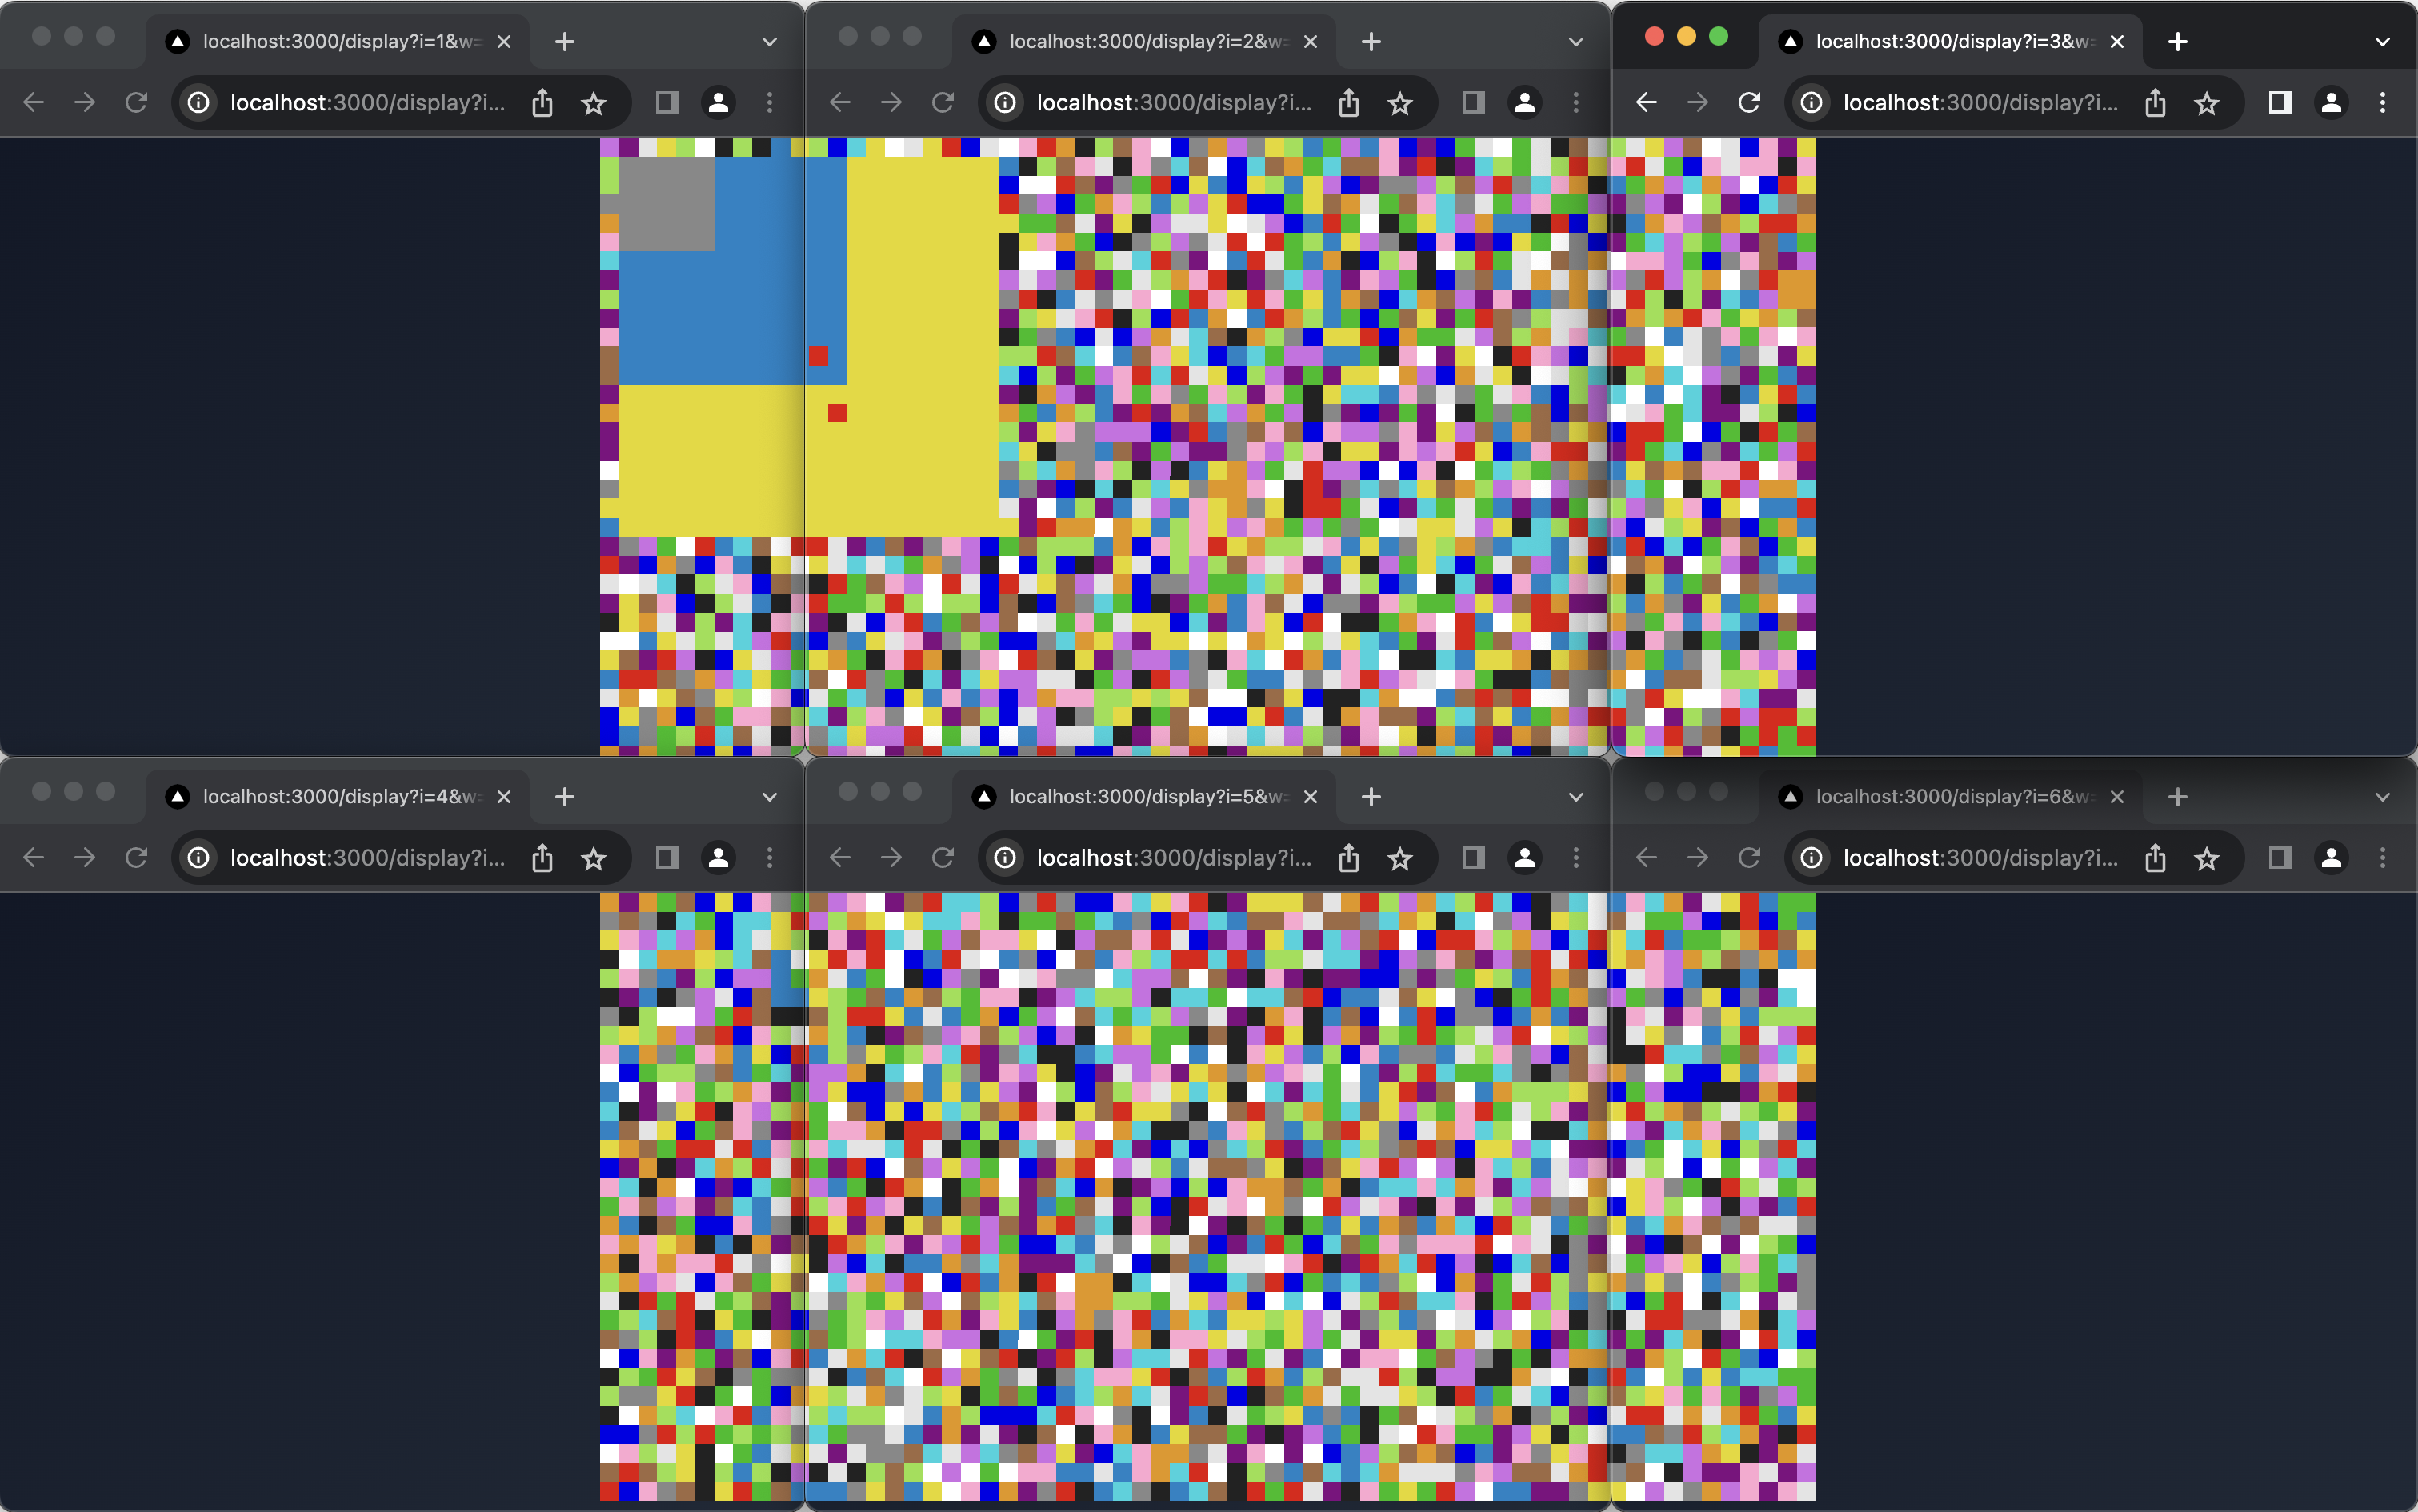
\includegraphics[width=1\textwidth]{./assets/figures/display-mode-example.png}
  \caption{Example d'affichage sur 6 écrans (6 fenêtres de navigateur)}
  \label{fig:display-mode-example}
\end{figure}

Dans le futur, il serait intéressant de pouvoir définir une taille de toile rectangulaire afin d'utiliser au mieux l'espace disponible sur les écrans. Comme cela n'était pas prévu dans le cahier des charges initial et qu'il faudrait modifier passablement l'application, cette fonctionnalité a été mise de côté pour après la fin du travail de Bachelor.

\subsection{Identification des utilisateurs}
La bonne identification des utilisateurs est un point crucial de l'application. En effet, il est nécessaire de pouvoir vérifier que les utilisateurs attendent bien le temps nécessaire avant de pouvoir placer un nouveau pixel. Pouvoir contourner cette règle casserait complètement le but principal de l'application qui est de faire collaborer les utilisateurs.

Ajouter une authentification classique avec un pseudonyme et un mot de passe ou même via un réseau social n'est pas souhaitable. En effet, cela ajouterait trop d'étapes à l'utilisateur avant de pouvoir placer un pixel. L'application a pour but d'être utilisée dans des milieux festifs, il faut donc que les usagers aient le moins de barrières possibles pour pouvoir l'utiliser.

Identifier les utilisateurs sans véritable authentification n'est pas trivial. L'idée est d'utiliser les empreintes digitales des joueurs, plus souvent appelées "fingerprint"~\cite{devicefingerprint}. Cela a pour but d'empêcher aux utilisateurs de contourner la règle du temps d'attente en rafraîchissant la page, en utilisant une navigation privée ou en changeant de navigateur par exemple. Cette méthode d'authentification se déroule quasiment uniquement dans le navigateur de l'utilisateur, du côté frontend. C'est la raison pour laquelle la phase d'identification est traitée dans cette section.

\subsubsection{Fingerprint}

Cette technique consiste à récupérer des informations sur le navigateur de l'utilisateur afin de créer un identifiant unique, notamment via les caractéristiques techniques de l'appareil comme sa résolution d'écran ou ses polices installées. La liste des attributs utilisés se doit d'être la plus grande possible afin d'éviter au maximum les collisions entre les utilisateurs. Un exemple plus détaillé sera présenté dans la prochaine sous-section. De plus, les informations doivent être stables afin que l'identifiant de l'utilisateur ne change pas. A partir de toutes ces caractéristiques, l'identifiant est créé via une fonction de hachage.

Ces méthodes demandent des algorithmes complexes et il est donc préférable d'utiliser une librairie existante. Malheureusement, le choix est limité. La librairie FingerprintJS~\cite{fingerprintjs} est la plus populaire mais possède une version propriétaire payante. L'idée de ce travail de Bachelor n'est pas de dépendre de multiples services tiers, que ce soit pour le déploiement ou pour le développement. C'est cette raison qui a poussé à chercher d'autres possibilités.

La seule vraie alternative open source se nomme Broprint.js~\cite{broprintjs}. Malheureusement, après quelques tests sur un échantillon d'une dizaine de personnes, des collisions d'identifiants ont déjà eu lieu car les ordinateurs potables étaient du même modèle. De plus, comme annoncé lors de la réalisation du POC \ref{poc-ameliorations}, certains utilisateurs avaient un identifiant différent à chaque chargement de la page, ce qui n'est pas acceptable

\subsubsection{FingerprintJS}
Le choix se tourne donc finalement vers FingerprintJS~\cite{fingerprintjs}. Il existe deux versions de la librairie, une gratuite et open source et la deuxième déjà mentionnée propriétaire. Ce qui permet de garder un code sans service tiers en utilisant la version open source. FingerprintJs annonce entre 40\% et 60\% de précision pour la version gratuite contrairement à la version payante qui tourne aux alentours de 99.5\%~\cite{fingerprintjsrepo}. Cette différence est due principalement au fait que la version gratuite contient uniquement du code exécuté côté client, sur le navigateur de l'utilisateur.

Afin d'avoir une idée des caractéristiques utilisées par FingerprintJS, un exemple de résultat~\cite{fingerprintjs-example} est donné sur leur site. La liste est conséquente, elle contient notamment:

\begin{itemize}
  \item Les polices installées, leurs préférences;
  \item Les réglages du navigateur comme sa langue, ses fonctionnalités activées ou pas etc;
  \item Les réglages de l'ordinateur comme le son, les couleurs, etc;
  \item Les informations sur la machine physique comme la résolution d'écran, le nombre de coeurs, la mémoire vive, etc.
\end{itemize}

En plus de toutes ces caractérisées, FingerprintJS utilise la notion de Canvas Fingerprint qui consiste à dessiner une image sur un canvas HTML5 (non affiché à l'utilisateur) et de récupérer le résultat sous forme de chaîne de caractères. Des variables comme le temps de rendu graphique sont utilisées afin de différencier chaque utilisateur.

Pour finir, l'avantage supplémentaire de FingerprintJS est que la version payante dispose d'un essai gratuit d'un mois et que la migration entre les deux versions concerne littéralement deux lignes~\cite{migratefingerprintjs}. Il suffit de changer le nom du package installé et d'ajouté la clé à notre compte FingerprintJS pour basculer sur la version payante. Il est donc envisageable d'utiliser la version gratuite en règle générale et de basculer sur la version payante lors des événements importants, comme le Baleinev festival. A noter qu'avec la version payante, les appels à l'API de FingerprintJS sont limités à 5 par seconde~\cite{fingerprintjs-limits}, ce qui n'est pas du tout conséquent. La version payante n'est donc pas forcément la meilleure solution pour les événements à grande échelle.

\subsubsection{Conclusion}

L'application actuelle avec la version gratuite de FingerPrintJS est fonctionnelle mais il est compliqué de savoir si les collisions d'identifiants sont fréquentes. Ce qui rend la situation peu idéale. De plus, des utilisateurs mal intentionnés pourraient utiliser des techniques pour envoyer une empreinte différente à chaque requête assez facilement afin de dessiner sans délai. Bloquer ce genre de comportement est difficile car il est impensable de limiter les requêtes par adresse IP. En effet, la majorité des étudiants sur le réseau de l'école partageraient la même adresse IP et ne pourraient donc pas dessiner en même temps. La solution serait d'ajouter une connexion avec un réseau social comme Google pour limiter les abus mais la perte en fluidité d'utilisation est conséquente. Cette question non triviale a été bien réfléchie est pourrait être donnée comme sujet d'un futur travail de Bachelor.

\section{Backend}

\subsection{Configuration}

Pour pouvoir modifier facilement la configuration de la toile, celle-ci est configurée grâce à des variables d'environnement du côté du backend. En effet, le backend transmet toutes ces valeurs au frontend lors de la première connexion comme expliqué dans la prochaine section \ref{section:communication-websockets}. Les variables d'environnement intéressantes sont présentées dans le listing \ref{listing:env-variables}.

\begin{listing}[H]
  \begin{minted}[linenos]{bash}
# The width and height of the board
BOARD_SIZE=64

# The time in seconds user need to wait before they can place another pixel
COOLDOWN=10

# Array of colors in hex format
COLORS='["#FFFFFF","#E4E4E4","#888888","#222222","#FFA7D1","#E50000","#E59500", ...]'

# The default stroke color index from the COLORS array
INITIAL_COLOR_INDEX=3

# The default zoom level
INITIAL_SCALE=9

# The number of pixels a user can place before they need to wait
MAX_PIXELS=3
\end{minted}
  \caption{Variables d'environnement de configuration de la toile}
  \label{listing:env-variables}
\end{listing}

En plus des variables présentées, d'autres plus classiques sont utilisées pour la connexion avec Redis ou choisir le port sur lequel tourne l'application par exemple.

\subsubsection{Validation des variables d'environnement}

Les variables par défaut sont définies dans un fichier \texttt{.env.defaults} qui sera copié dans un fichier \texttt{.env} lors de l'installation du projet. Ce fichier \texttt{.env} est utilisé et chargé par le backend et n'est pas versionné sur le répertoire git. En plus de ces deux fichiers, un troisième est défini appelé \texttt{.env.schema}. Ce fichier contient la liste des variables d'environnement ainsi que leur structure sous la forme d'une Regex. Ce fichier est utilisé par le package \texttt{dotenv-extended}~\cite{dotenv-extended} qui permet de valider les variables d'environnement. Si une variable d'environnement est manquante ou si sa valeur ne correspond pas à la Regex définie dans le fichier \texttt{.env.schema}, la pipeline de CI/CD ainsi qu'Husky en local ne passeront pas. Cela permet d'éviter les erreurs inutiles lorsqu'un développeur ajoute ou modifie une variable d'environnement.

\subsection{Communication WebSockets}
\label{section:communication-websockets}

\subsubsection{Connexion initiale}

\fig[H, width=0.9\textwidth]{Diagramme de séquence de la connexion WebSockets}{sequence-websockets-connection.svg}

Comme démontré dans la figure \ref{sequence-websockets-connection.svg}, le frontend initialise la connexion WebSocket avec le backend. Il génère ensuite son identifiant unique, sa fingerprint, et l'envoie à l'aide de l'événement \texttt{JOIN} au backend. Le backend stocke ensuite cet identifiant dans le Socket utilisé pour la connexion avec ce client pour que le client n'ait pas besoin de l'envoyer à chaque nouvelle requête. Le backend répond ensuite au frontend en lui envoyant la configuration de la toile, son état initial, les couleurs disponibles, etc. Il envoie également le potentiel temps d'attente actuel de l'utilisateur avant de pouvoir reposer un pixel.

Une fois cet état initial reçu et stocké du côté du frontend, la toile est affichée. Le client peut ensuite envoyer des événements pour poser des pixels et le serveur enverra lui des événements pour notifier le client de changements sur la toile réalisés par d'autres utilisateurs comme démontré dans la figure \ref{sequence-websockets-pixels.svg}.

\subsubsection{Pose de pixels}

\fig[H, width=0.8\textwidth]{Diagramme de séquence de la pose d'un pixel}{sequence-websockets-pixels.svg}

Le déroulement de la pose d'un pixel est assez intuitif. Le client qui pose le pixel envoie un événement \texttt{PIXEL\_FROM\_PLAYER} au serveur avec les coordonnées et la couleur du pixel. Le serveur vérifie que l'utilisateur est autorisé à réaliser cette action avant de stocker le nouveau pixel comme la prochaine section \ref{section:stockage} l'explique. Le serveur envoie ensuite s'il y a eu des modifications un événement \texttt{UPDATE\_BOARD} chaque 100 millisecondes à tous les clients connectés pour qu'ils mettent à jour leur toile avec les nouveaux pixels.

La subtilité se trouve dans le fait que le client qui a placé le pixel va en réalité le dessiner deux fois sur le canvas: immédiatement lors de son clique sur le bouton "Place" ainsi qu'à la réception de l'événement \texttt{UPDATE\_BOARD}. Cela permet d'avoir un retour instantané pour l'utilisateur qui a posé le pixel, sans devoir prendre en compte une potentielle latence du serveur.

\subsection{Stockage de l'état actuel de la toile}
\label{section:stockage}

Redis offre de nombreuses manières de stocker des données. La première option est de stocker chaque couleur de pixel dans une clé en utilisant les coordonnées (x, y) comme clé. Cependant, récupérer un nombre important de clés en une fois (lors du chargement initial de la toile) n'est pas efficace. En effet, il faut scanner les différentes clés en spécifiant un paterne à trouver. Il est donc préférable de stocker l'état de la toile dans une seule clé Redis. Pour cela, il est possible d'utiliser le type de données Bitfield~\cite{bitfield} de Redis. Ce type de données permet de stocker des bits dans une clé Redis et toutes les opérations se font en \bigO{1}. Il s'agit de la structure de données utilisée par l'équipe de \gls{reddit} dans leurs applications r/place de 2017 et 2022. Le Senior Software Engineer de \gls{reddit} Daniel Ellis a notamment donnée une conférence expliquant leur utilisation de Redis lors de la RedisConf 17~\cite{redisconf}. L'implémentation qui suit est donc basée sur les informations données dans cette conférence.

Afin de convertir la toile en une suite de bits, il est nécessaire de donner un ID à chaque couleur afin de ne pas stocker un nombre incalculable de chaîne de caractères correspondant aux différentes couleurs. Pour avoir une marge concernant le nombre de couleurs disponibles, le type de chaque élément du Bitfield a été spécifié comme un entier non signé sur 8 bits. Cela permet de stocker 256 couleurs à la place des maximum 16 disponibles avec 4 bits. Le second avantage à utiliser 8 bits et qu'il rend possible l'utilisation d'un Uint8ClampedArray~\cite{uint8clampedarray} du côté du client afin de créer une image du contenu du canvas très simplement sans avoir à faire de conversion.

Pour calculer l'offset du bit à modifier en fonction de la position du pixel (x, y), il est possible d'utiliser la simple formule suivante:
\begin{equation}
  \mathrm{offset} = (y * width + x)
\end{equation}

Pour avoir accès l'entièreté du canvas, il suffit de récupérer la clé Redis sans préciser d'offset. Il est ainsi possible d'avoir accès à un tableau d'entiers représentant les couleurs de chaque pixel de la toile.

\subsection{Stockage de l'historique}

Comme précisé précédemment, le Bitfield Redis n'a aucune idée des états passés de chaque pixel. De plus, il ne contient aucune information concernant la date ou l'utilisateur ayant posé le pixel. La conception de ces données a été réalisée dans une table SQL unique nommée \texttt{pixel} contenant les champs suivants:

\begin{itemize}
  \item \texttt{id}: identifiant unique de la pose du pixel;
  \item \texttt{x}: position x du pixel;
  \item \texttt{y}: position y du pixel;
  \item \texttt{color}: couleur du pixel en hexadécimal;
  \item \texttt{created\_at}: date et heure à laquelle le pixel a été posé;
  \item \texttt{user\_id}: identifiant de l'utilisateur ayant posé le pixel;
\end{itemize}

La valeur hexadécimal de la couleur est stockée à la place de l'identifiant de la couleur car les couleurs peuvent varier au fil du temps. Il est donc nécessaire de stocker sa valeur à la pose du pixel pour avoir un historique correct.

Initialement, un booléen \texttt{is\_admin} permettait de savoir si l'utilisateur qui a posé le pixel est un administrateur ou non. Il a été jugé inutile, en effet il suffit d'utiliser un identifiant comme \texttt{"ADMIN"} dans le champ \texttt{user\_id} pour identifier les actions de modération à la place d'une FingerPrint.

\subsection{Gestion de la durée d'attente entre la pose de pixels}

Redis est également utilisé pour vérifier que le temps d'attente entre chaque pixel est bien respecté pour chaque utilisateur. En effet, il est possible de stocker des données dans Redis avec une durée de vie, qui correspond ici au temps d'attente.

Chaque utilisateur est stocké selon le format de clé suivant: \mintinline[breaklines]{bash}{users:<fingerprint>}. La clé aurait simplement pu être la fingerprint de l'utilisateur mais la préfixer avec \texttt{users:} permet de pouvoir sélectionner rapidement toutes les clés des utilisateurs via un scan. Cela peut être utile pour la remise à zéro des temps d'attente ou simplement pour vider le cache sans risquer de toucher à l'état de la toile. Concernant la valeur associée à la clé, il s'agit simplement du nombre de pixels posés par l'utilisateur durant l'intervalle. S'il s'agit du premier pixel, la clé est créée et le temps d'attente démarre. Pour les pixels suivants, la valeur est incrémentée grâce aux méthodes que Redis nous offre. Si le nombre de pixels stockés est égal au nombre maximal de pixels autorisés, l'opération est simplement refusée.

\subsection{Administration}
\label{section:administration}

Pour protéger les actions réalisables uniquement par des administrateurs, une authentification doit être mise en place. L'implémentation se base sur le module Passport~\cite{passport} qui est le standard en matière d'authentification dans le monde \gls{nodejs}. Passport propose des centaines de manières de s'authentifier, appelées "stratégies". Celle choisie se nomme HeaderAPIKey~\cite{passport-headerapikey} et permet de vérifier qu'une clé d'API est présente dans les entêtes de la requête HTTP. Cette clé est ensuite comparée à la valeur stockée comme variable d'environnement \mintinline[breaklines]{bash}{API_KEY}. Si la clé est correcte, l'utilisateur est considéré comme authentifié et peut effectuer les actions réservées aux administrateurs.

Cette stratégie d'authentification par clé d'API est choisie pour sa facilité d'implémentation. En effet, aucun stockage de session ou même dans une base de données n'est nécessaire. De plus, les besoins d'administration sont très simples pour l'instant et ne nécessitent pas plus que de simples appels HTTP.

Dans les fonctionnalités "nice-to-have" du cahier du charges, il était question de réaliser un dashboard pour faciliter les tâches d'administration. Malheureusement, le temps a manqué pour implémenter cette tâche lors de ce travail de Bachelor. Ce dashboard sera donc réalisé dans le futur et les administrateurs utiliseront pour l'instant les appels HTTP.

\subsubsection{Remise à zéro de la toile}

Le listing \ref{listing:http-call-reset-board} démontre des appels HTTP en ligne de commande sur la route permettant de remettre à zéro la toile pour tous les utilisateurs. Lorsque la clé d'API est incorrecte ou absente, une erreur 401 est retournée nous signifiant que l'utilisateur n'est pas autorisé à effectuer cette action.

\begin{listing}[h]
  \begin{minted}[breaklines]{bash}
  # Version sans clé dans l'entête ou clé incorrecte
  curl -X POST http://localhost:4000/board/reset
  {"statusCode":401,"message":"Unauthorized"}%

  # Version avec clé correcte dans l'entête
  curl -X POST http://localhost:4000/board/reset --header "apiKey: API_KEY"
  {"status":"ok","message":"Board reset"}%
\end{minted}
  \caption{Appels HTTP pour remettre à zéro la toile}
  \label{listing:http-call-reset-board}
\end{listing}

Grâce à l'implémentation de l'authentification sous la forme d'un décorateur \gls{typescript}~\cite{typescript-decorators}, il est possible de protéger simplement les méthodes souhaitées. En effet, les décorateurs permettent d'ajouter des fonctionnalités à une méthode sans avoir à la modifier, en s'injectant directement dans le contexte de celle-ci. Par exemple, la méthode permettant de remettre à zéro la toile est protégée par le décorateur \texttt{ApiKeyAuth} qui vérifie que la bonne clé d'API est présente dans les entêtes de la requête HTTP comme le montre le listing \ref{listing:admin-methods-auth}.

\begin{listing}[h]
  \begin{minted}[breaklines, highlightlines={2}, linenos]{typescript}
@Post()
@ApiKeyAuth()
async reset() {
  await this.boardGateway.resetBoard();

  return {
    status: 'ok',
    message: 'Board reset',
  };
}
\end{minted}
  \caption{Protection des méthodes d'administration par décorateur}
  \label{listing:admin-methods-auth}
\end{listing}

La méthode \texttt{resetBoard} du BoardGateway supprime simplement la clé Redis contenant l'état complet de la toile. De plus, tous les utilisateurs connectés sur l'application sont notifiés de la remise à zéro de la toile grâce à un événement WebSockets et leur canvas est vidé. Cela permet de ne pas avoir à recharger la page pour voir la toile se vider. Ce qui n'aurait pas été pratique car le but principal de cette fonctionnalité et de censurer rapidement les oeuvres inappropriées.

\subsubsection{Censurer une partie de la toile}

Il est également possible pour les administrateurs de censurer une zone de la toile, afin de ne pas perdre l'entièreté des oeuvres. Il suffit de passer en paramètre de l'appel HTTP les coordonnées des coins supérieur gauche et inférieur droit de la zone à censurer ainsi qu'une potentielle couleur à utiliser pour remplir la zone. Si aucune couleur n'est passée en paramètre, la zone est remplie de blanc. En attendant l'implémentation du dashboard pour faciliter cette tâche, l'administrateur peut récupérer les coordonnées directement depuis le frontend de l'application.

Le backend va ensuite générer tous les pixels se trouvant dans la zone et les insérer dans le Bitfield Redis ainsi que dans la base de données avant d'en informer tous les utilisateurs via WebSocket. Il aurait été possible d'appeler la méthode utilisée précédemment pour stocker un pixel pour tous les pixels de la zone. Cependant, cette approche n'aurait pas été très efficace. Il est préférable de réaliser ces tâches en parallèle afin d'accélérer le processus comme le montre le listing \ref{listing:admin-reset-area}.

\begin{listing}[h]
  \begin{minted}[breaklines, linenos]{ts}
  private async storePixelInBitfield(pixel: Pixel) {
    const { x, y, color } = pixel;
    const offset = y * this.configService.get(BOARD_SIZE) + x;
    return this.redisClient.bitfield(
      BOARD_KEY,
      'SET',
      UINT_8,
      `#${offset}`,
      color,
    );
  }

  async resetArea(pixels: Pixel[]) {
    // Store in Redis
    const promises = pixels.map((pixel) => this.storePixelInBitfield(pixel));
    await Promise.all(promises);

    // Store in Database
    const colors = this.configService.get(COLORS);
    await this.prisma.pixel.createMany({
      data: pixels.map((pixel) => ({
        x: pixel.x,
        y: pixel.y,
        color: colors[pixel.color],
        userId: 'ADMIN',
      })),
    });
  }
\end{minted}
  \caption{Réinitialisation d'une zone de la toile}
  \label{listing:admin-reset-area}
\end{listing}

De plus, utiliser la méthode \texttt{createMany} de Prisma permet d'effectuer un seul appel à la base de données pour insérer tous les pixels de la zone. Cela permet d'éviter de surcharger la base de données avec de nombreux appels.

\subsubsection{Mode lecture seule}

La dernière action disponible pour les administrateurs est la possibilité de passer la toile en mode lecture seule. Cette option peut être intéressante si le comportement des utilisateurs devient trop problématique en fin de soirée par exemple. Cela permet de ne pas perdre les oeuvres déjà réalisées.

L'implémentation côté backend est simple. Il s'agit d'un attribut booléen stocké dans l'instance de la classe \texttt{BoardGateway}. Lorsque celui-ci est à \texttt{true}, la méthode \texttt{addPixel} ne fait rien. A chaque fois que ce booléen est modifié, sa nouvelle valeur est envoyé à tous les utilisateurs via WebSocket.

L'interface de l'utilisateur se met à jour directement à la réception de la nouvelle valeur. Si la toile est en lecture seule, l'application affiche la version de la toile normalement utilisée dans le mode affichage discuté dans la section \ref{display-mode}. Cela permet d'empêcher facilement aux utilisateurs de modifier la toile en enlever simplement l'interface de pose de pixel.

De plus, un message indiquant aux utilisateurs que la toile se trouve en lecture seule est affiché afin de les informer de la situation. Cela permet d'éviter de la frustration s'ils pensent que l'application ne fonctionne pas correctement.

\section{Package}

Afin d'éviter la duplication de code lorsque celui-ci est utilisé à la fois du côté du frontend ainsi que du backend, il est nécessaire de trouver un moyen de partager du code entre les deux applications. Les deux applications utilisent TypeScript, ce qui rend la tâche plus simple. Cependant, de nombreuses façons de faire sont disponibles et il est nécessaire de choisir la plus adaptée à ce cas d'utilisation.

\subsection{Solutions d'implémentation possibles}

\subsubsection{Vrai package npm}

Comme le monorepo utilise \gls{pnpm}, il est possible de créer un package et d'ensuite le référencer dans les fichiers \mintinline[breaklines]{bash}{package.json} des deux applications sans devoir le publier sur un registre. C'est d'ailleurs cette solution qui a été choisie pour l'application Pimp My Wall existante. Cependant, cette manière de faire nécessite de réaliser un build du package après chaque modification du code TypeScript, ce qui est loin d'être idéal en terme de productivité.

\subsubsection{Project References}

Les Project References~\cite{project-references} sont une fonctionnalité TypeScript qui correspondent parfaitement aux besoin du projet d'un point de vue théorique. En ajoutant au fichier de configuration TypeScript (\mintinline[breaklines]{bash}{tsconfig.json}) de l'application une référence vers le package, le compilateur va automatiquement compiler le package avant de compiler l'application. Mais le problème est le suivant: cette fonctionnalité n'est disponible que sur le compilateur officiel de Typescript, tsc~\cite{tsc} en utilisant le flag \mintinline[breaklines]{bash}{--build}. Malheureusement, aussi bien Next.js que Nest.js utilisent des compilateurs TypeScript personnalisés qui ne supportent pas cette fonctionnalité~\cite{nest-tsc-build-option}. Il n'est donc pas possible d'utiliser cette fonctionnalité sans devoir réaliser des solutions maisons peu maintenables ou élégantes.

\subsubsection{Internal Package}

Le blog de Turbo~\cite{you-might-not-need-typescript-project-references}, un outil permettant également de faciliter la gestion des monorepos, propose une solution innovante à ce problème de code partagé: les internal packages. Il s'agit de packages qui ne contiennent pas de fichier \mintinline[breaklines]{bash}{tsconfig.json}. De plus, ils se contentent d'exporter directement les fichiers TypeScript dans leur fichier \mintinline[breaklines]{bash}{package.json} à la place des fichiers JavaScript transpilés.

\begin{listing}[H]
  \begin{minted}[breaklines, linenos]{json}
  {
    "name": "@beescreens/beeplace"
    "main": "./src/index.ts", // instead of "./dist/index.js"
    "types": "./src/index.ts", // instead of "./dist/index.d.ts",
    "dependencies": {
      // ...
    },
    "devDependencies": {
      // ...
    }
  }
\end{minted}
  \caption{Exemple de \texttt{package.json} d'un internal package}
  \label{listing:internal-package-json}
\end{listing}

Cette solution est idéale car très facile à mettre en place. Cependant, il est nécessaire que les applications qui consument le package transpilent le code TypeScript. En effet, le code TypeScript ne peut pas être exécuté directement une fois importé, il doit être transpilé avec le reste de l'application. Next.js permet cette option en ajoutant le package à transpiler dans la configuration du framework comme le montre le listing \ref{listing:next-transpile-package}.

\begin{listing}[H]
  \begin{minted}[breaklines, linenos]{javascript}
  /** @type {import('next').NextConfig} */
  const nextConfig = {
    transpilePackages: ['@beescreens/beeplace'],
  };
  module.exports = nextConfig;
\end{minted}
  \caption{Modification de la configuration Next pour transpiler un package}
  \label{listing:next-transpile-package}
\end{listing}

Malheureusement, ce n'est pas le cas de Nest.js. Nest n'a pas de compilateur dédié en dehors du compilateur TypeScript. Il faudrait ajouter un utilitaire comme Webpack~\cite{webpack} qui s'occuperait de transpiler le code TypeScript du package. Cependant, cela ajouterait une complexité assez conséquente au projet et une maintenabilité réduite. Il est donc préférable de trouver une autre solution.

\subsubsection{Path alias}

Une autre solution est d'importer directement dans l'application souhaitée le code TypeScript du package. Bien entendu, les chemins relatifs seraient assez peu agréables et maintenables. Heureusement, TypeScript propose de créer des Path alias dans le fichier de configuration \mintinline[breaklines]{bash}{tsconfig.json}.

\begin{listing}[H]
  \begin{minted}[breaklines, linenos]{json}
  "paths": {
    "@/*": ["./src/*"],
    "@beescreens/beeplace": ["../common/src/index"]
  }
\end{minted}
  \caption{Path alias dans le fichier de configuration TypeScript \texttt{tsconfig.json}}
  \label{listing:path-alias-tsconfig}
\end{listing}

L'application a donc directement accès au fichier \mintinline[breaklines]{bash}{index} du package qui s'occupe d'exporter tout le code en commun.

Cependant, une subtilité apparaît pour faire fonctionner cette solution. Il faut annoncer au compilateur Next.js que le projet utilise des fichiers en dehors du dossier de l'application en elle-même. Autrement, le code du package ne sera pas transpilé et une erreur apparaîtra au lancement de l'application.

\begin{listing}[H]
  \begin{minted}[breaklines, linenos]{javascript}
  /** @type {import('next').NextConfig} */
  const nextConfig = {
    experimental: {
      externalDir: true,
    },
  };
  module.exports = nextConfig;
\end{minted}
  \caption{Modification de la configuration Next pour gérer le path alias}
  \label{listing:next-external-dir}
\end{listing}

Du côté de Nest, le package est automatiquement transpilé et ajouté au dossier de build \mintinline[breaklines]{bash}{.nest}. Cependant, cela change la hiérarchie des dossiers une fois build et il faut donc préciser à Nest quel fichier exécuter au lancement de l'application. Cette configuration se fait facilement dans le fichier \mintinline[breaklines]{bash}{nest-cli.json}.

\begin{listing}[H]
  \begin{minted}[breaklines, linenos]{json}
  {
    // ...
    "entryFile": "backend/src/main"
    // ...
  }
\end{minted}
  \caption{Modification de la configuration Nest pour gérer le path alias}
  \label{listing:nest-entry-file}
\end{listing}

\subsubsection{Solution choisie}

Le choix s'est donc finalement tourné vers les path alias. En dehors des quelques subtilités à connaître, cette solution est très simple à mettre en place et à maintenir. De plus, elle permet d'avoir une expérience de développement agréable en évitant d'avoir à build le code à chaque modification.

Pour conclure, il ne s'agit plus vraiment d'un package à proprement parler mais plutôt d'un simple dossier partagé entre les deux applications. En effet, il n'est plus build indépendamment ni importé dans les fichiers \mintinline[breaklines]{bash}{package.json} des applications respectives. Ces raisons ont poussé à renommer le dossier en \mintinline[breaklines]{bash}{common} et le déplacer à côté des deux applications dans le répertoire beeplace:

\begin{listing}[H]
  \begin{tcolorbox}[arc=0mm,colback=white!5!white]
    \dirtree{%
      .1 /.
      .2 apps.
      .3 beeplace.
      .4 backend.
      .4 common.
      .4 frontend.
      .3 ....
      .2 ....
    }
  \end{tcolorbox}
  \caption{Structure du répertoire de l'application BeePlace avec le code partagé}
  \label{listing:beeplace-repo-structure-v2}
\end{listing}

\subsection{Code partagé}

Le code en commun contient majoritairement deux catégories de code:

\begin{itemize}
  \item Des types TypeScript qui seront supprimés du code lors de la transpilation en JavaScript;
  \item Des énumérations TypeScript qui seront transformées en objets dans le code JavaScript.
\end{itemize}

Il aurait également été possible d'ajouter par exemple des fonctions utilitaires ou des classes en commun. Cependant, ce besoin n'est pas apparu durant le développement du projet.

\subsubsection{Types}

Les types partagés sont par exemple l'interface représentant un pixel ou encore l'état initial reçu par le client lors de la connexion à l'application comme le montre le listing \ref{listing:shared-types}.

\begin{listing}[H]
  \begin{minted}[breaklines, linenos]{ts}
    export interface Coordinate {
      x: number;
      y: number;
    }

    export interface Pixel extends Coordinate {
      color: number;
    }

    export interface InitialState {
      board: number[];
      canvasSize: number;
      colors: string[];
      cooldown: number;
      initialColor: number;
      // ...
    }
\end{minted}
  \caption{Exemples de types partagés entre le backend et le frontend}
  \label{listing:shared-types}
\end{listing}

\subsubsection{Enumérations et événements WebSockets}

Des énumérations sont utilisées pour représenter les événements WebSockets. Il en existe deux catégories: les événements envoyés par le client \texttt{ClientEvent} et les événements envoyés par le serveur \texttt{ServerEvent}.

\begin{listing}[H]
  \begin{minted}[breaklines, linenos]{ts}
    export enum ServerEvent {
      READ_ONLY = 'readOnly',
      RESET_BOARD = 'resetBoard',
      UPDATE_BOARD = 'u', // shortest possible name to reduce bandwidth usage for end users
      USER_COUNT = 'userCount',
    }

    export enum ClientEvent {
      JOIN = 'join',
      PIXEL_FROM_PLAYER = 'pixelFromPlayer',
    }
\end{minted}
  \caption{Énumérations des événements WebSockets}
  \label{listing:websocket-events-enums}
\end{listing}

Par la suite, ces énumérations sont utilisées dans le code des deux applications mais également dans le code commun. En effet, depuis Socket.IO 3, il est possible de typer complètement les événements WebSocket. Il suffit de créer des interfaces pour chaque événement, en typant les paramètres et le retour de la fonction.

\begin{listing}[H]
  \begin{minted}[breaklines, linenos]{ts}
    interface ServerToClientEvents {
      [ServerEvent.READ_ONLY]: (readOnly: boolean) => void;
      [ServerEvent.RESET_BOARD]: () => void;
      [ServerEvent.UPDATE_BOARD]: (data: string) => void;
      [ServerEvent.USER_COUNT]: (count: number) => void;
    }

    interface ClientToServerEvents {
      [ClientEvent.JOIN]: (
        fingerprint: string,
        callback: (response: JoinResponse) => void,
      ) => void;
      [ClientEvent.PIXEL_FROM_PLAYER]: (pixel: Pixel) => void;
    }
\end{minted}
  \caption{Interfaces des événements WebSockets}
  \label{listing:websockets-events-interfaces}
\end{listing}

Pour finir, il suffit d'utiliser ces interfaces dans les types fournis par Socket.IO afin d'exposer les versions typées des sockets pour le client et le serveur Socket.IO. Il est également possible de typer le \texttt{SocketData}, un objet de stockage propre à chaque instance de Socket côté serveur. Celui-ci est utilisé pour stocker la Fingerprint associée au client dans le cas de \gls{beeplace}.

\begin{listing}[H]
  \begin{minted}[breaklines, linenos]{ts}
    interface SocketData {
      fingerprint: string;
    }

    export type BeePlaceFrontendSocket = ClientSocket<
      ServerToClientEvents,
      ClientToServerEvents
    >;
    export type BeePlaceBackendSocket = Socket<
      ClientToServerEvents,
      ServerToClientEvents,
      SocketData
    >;
\end{minted}
  \caption{Sockets client et serveur Socket.IO typés}
  \label{listing:typed-socket-io}
\end{listing}

Les applications utilisent donc ces Sockets typées dans leur code respectif. Cela permet d'avoir une très bonne expérience pour le développeur. Il lui suffit d'utiliser l'énumération des événements disponibles et tout le reste de la fonction sera typé automatiquement. Cela évite notamment les erreurs basiques lorsque le code est modifié à un endroit mais pas dans les autres occurrences.
